%%%%%%%%%%%%%%%%%%%%%%%%%%%%%%%%%%%%%%%%%%%%%%%%%%%%%%%%%%%%%%%%%%%%%%
% How to use writeLaTeX: 
%
% You edit the source code here on the left, and the preview on the
% right shows you the result within a few seconds.
%
% Bookmark this page and share the URL with your co-authors. They can
% edit at the same time!
%
% You can upload figures, bibliographies, custom classes and
% styles using the files menu.
%
%%%%%%%%%%%%%%%%%%%%%%%%%%%%%%%%%%%%%%%%%%%%%%%%%%%%%%%%%%%%%%%%%%%%%%

\documentclass[12pt]{article}

\usepackage{sbc-template}

\usepackage{graphicx,url}

\usepackage[brazil]{babel}   
\usepackage[utf8]{inputenc}  

     
\sloppy

\title{Paralelização para memória distribuída com MPI}

\author{Bruno C. P. D. Rosa, Cristofer A. Oswald}

\address{Departamento de informática 
  \\Centro de Tecnologia -- Universidade Estadual de Maringá
  (UEM)\\
  Maringá -- PR -- Brasil
}

\begin{document} 

\maketitle
     
\begin{resumo} 
  A busca continua por mais poder computacional e eficiência levou a inevitável ascensão das arquiteturas paralelas, que atualmente dominam o mercado e estão presentes em todo tipo de dispositivo. Estas mudanças também afetaram profundamente o modelo de programação, causando uma troca de paradigma. Programar paralelamente se tornou crucial para o desenvolvimento de aplicações capazes de utilizar o hardware moderno. Neste trabalho, fazemos uso da interface de passagem de mensagens MPI, que será utilizada para realizar experimentos com memória distribuída em diversos computadores juntamente da biblioteca pthreads (posix threads), utilizada para paralelizar os fluxos em cada um dos computadores, tornando a implementação híbrida. Para os testes foi utilizado o algoritmo Fast da CAP benchmark como objeto de testes.
\end{resumo}


\section{Introdução}
Na história da ciência da computação os avanços no hardware sempre foram os maiores impulsionadores do aumento do poder computacional, o mesmo software simplesmente roda mais rápido à medida que os processadores apresentam uma maior velocidade de processamento, durante anos cientistas e desenvolvedores de software contaram com isto para atingirem seus objetivos. Esse impulso, porém, vem diminuindo desde 2003 devido a questões de consumo de energia e dissipação de calor, que limitaram o aumento da frequência do clock e o nível de tarefas que podiam ser realizadas em cada período de clock dentro de uma única CPU \cite{kirk2011programming}. A indústria de microprocessadores respondeu a estas limitações com a mudança do paradigma dominante nas arquiteturas de computadores, que agora são as arquiteturas paralelas, principalmente sob a forma de processadores multinúcleos.

Um dos métodos de paralelização mais antigos é a paralelização para execução em cluster, onde cada fluxo de execução é alocado em uma máquina diferente num cluster de computadores. Assim cada máquina se torna responsável por parte do processamento, esta estratégia já era utilizada muito antes do surgimento dos processadores multinúcleos. Este modelo, denominado programação paralela com memória distribuída, apresenta vantagens e desvantagens quando comparado ao modelo de paralelização com memória compartilhada. Em um trabalho realizado previamente exploramos os aspectos deste modelo utilizando a técnica de passagem de mensagens utilizando MPI como solução para comunicação entre os dispositivos.

Neste trabalho propomos a utilização da técnica programação paralela com memória compartilhada em conjunto com a programação com memória distribuída. Este modelo que une as técnicas pode ser chamado de programação paralela hibrida. Para a implementação de um programa neste paradigma optamos por utilizar \textit{posix threads} (pthreads) como solução para memória compartilhada e, como no trabalho anterior, MPI como solução para memória distribuída, tendo como objetivo final analisar o desempenho do modelo hibrido.


\section{Projeto} \label{sec:projeto}

O programa de alto desempenho \textit{Fast} escrito na linguagem C, foi escolhido para ser usado como objeto de experimentação deste trabalho. A versão original do programa é uma implementação paralela do algoritmo utilizando a técnica de paralelização de laços com a ferramenta \textit{OpenMP}. \textit{Fast} faz parte do CAP benchmark \cite{souza2017cap}, um benchmark desenvolvimento com o objetivo principal de testar o desempenho e o gasto de energia em processadores multinúcleos. O número de fluxos de execução concorrentes e o tamanho do problema são parâmetros de execução do programa.

\textit{Fast}, acrônimo do inglês \textit{Features from Accelerated Segment Test} implementa um método para detecção de cantos em imagens seguindo o padrão estêncil paralelo. É comumente usado para extrair características e mapear objetos em tarefas de visão computacional. Em sua execução, um circulo de 16 pixels é utilizado para testar se um ponto \(p\) candidato é um canto ou não. Um valor inteiro de 1 a 16 é atribuído para cada pixel no circulo em ordem horária. Se todos os \(N\) pixel contínuos do circulo são mais claros que a intensidade do pixel candidato \(p\) somado a um valor limiar \(t\) ou todos mais escuros que a intensidade de \(p - t \), então \(p\) é classificado como um canto.
	
Para avaliar o desempenho do programa no modelo paralelo com memória hibrida foi implementada uma versão que utiliza a técnica de passagem de mensagens através de MPI e a paralelização a nível local com pthreads. Uma implementação MPI (\textit{Message Passing Interface}) é uma API para envio de mensagens juntamente de protocolos e especificações semânticas sobre seu funcionamento \cite{Lusk96ahigh-performance}. A implementação MPI utilizada é a Open MPI, uma versão desenvolvida e mantida por um consórcio de parceiros acadêmicos, pesquisadores e outros interessados. A API Open MPI disponibiliza funções para inicialização do ambiente de execução, envio e recebimento de mensagens entre outras funções como diretivas de sincronização da execução. A biblioteca de threads utilizada implementa o padrão posix threads, tradicionalmente utilizado para programação paralela em ambientes linux.

 A estratégia \textit{Mestre-Escravo} foi adotada como modelo de comunicação no desenvolvimento do programa. Neste contexto, o processo principal, intitulado como Mestre, se encarrega de executar tarefas de inicialização do programa como alocação da matriz de pixels, preenchimento aleatório da mesma, envio dos dados para os processos Escravos e recebimento dos resultados computados por eles. Os demais processos, intitulados Escravos, são os processos que irão realizar, de maneira coletiva, a computação efetiva do programa. Estes iniciam sua execução aguardando o recebimento da mensagem do processo Mestre contendo os dados os quais irão computar, executam o método de detecção de cantos sob a sub-área recebida e retornam, na forma de mensagem, o resultado obtido, neste caso o número de cantos encontrados. Todos os envios e recebimentos de dados realizados entre o Mestre e os Escravos ocorrem através de métodos MPI para envio de mensagens, citados anteriormente. Nota-se que no modelo de comunicação adotado a troca de mensagens ocorre exclusivamente entre o processo Mestre para os demais, ou seja, processos Escravos não se comunicam entre eles.

Todos os códigos foram compilados com o compilador \textit{mpicc} parte do Open MPI com otimização O3. As execuções do experimento foram realizadas no laboratório Lin 2 do Departamento de Informática da Universidade Estadual de Maringá em oito computadores com configurações semelhantes executando sistema operacional Ubuntu. Os dados coletados para a avaliação compreendem os resultados de execuções.

\section{Avaliação}

Para garantir resultados mais precisos e evitar possíveis falsas conclusões, a avaliação de speedup contempla execuções com quantidades diferentes de fluxos de execução concorrentes (de 2 a 16), sendo que cada uma das configurações foi executada 11 vezes, assim, a primeira, que tem a finalidade de aquecer a cache, o melhor e o pior resultados são descartados, dessa maneira, os dados utilizados na avaliação são as médias das 8 execuções restantes. A entrada do problema selecionada para a realização dos experimentos é uma entrada 33\% maior que a maior entrada implementada no programa original. Planejava-se a utilização da ferramenta MPIP para obtenção de dados sobre a troca de mensagens, entretanto, apesar de ter sido utilizada no trabalho anterior na implementação deste trabalho não foi possível sua execução pois ela apresentou erros com a implementação utilizando pthreads.

Sobre a quantidade de fluxos concorrentes, é importante notar que o número de máquinas usadas variou entre as configurações e que as execuções sempre contaram com um processo a mais, pois o processo Mestre não é contabilizado na quantidade de fluxos. Diferentemente da implementação do trabalho anterior, neste trabalho cada máquina executa apenas um processo, exceto a máquina principal que abriga, adicionalmente, o processo Mestre. A execução desta forma é paralelizada através das threads lançadas em cada máquina, assim temos a quantidades de máquinas e fluxos como: 

\begin{itemize}
\item \textbf{2 fluxos:} uma máquina com duas threads.
\item \textbf{4 fluxos:} duas máquinas com duas threads por máquina.
\item \textbf{8 fluxos:} quatro máquinas com duas threads por máquina.
\item \textbf{16 fluxos:} oito máquinas com duas threads por máquina.
\item \textbf{32 fluxos:} oito máquinas com quatro threads por máquina.
\end{itemize}

\newpage
\subsection{Speedup}

Como foco principal deste trabalho, utilizou-se os resultados dos experimentos para avaliar o impacto da paralelização com o modelo de memória hibrida. O gráfico de speedup da figura 1 é composto por três componentes: Speedup ideal, Speedup obtido desconsiderando o overhead e por fim Speedup real considerando overhead, este overhead será explicado posteriormente.

\begin{figure}[ht!]
\centering
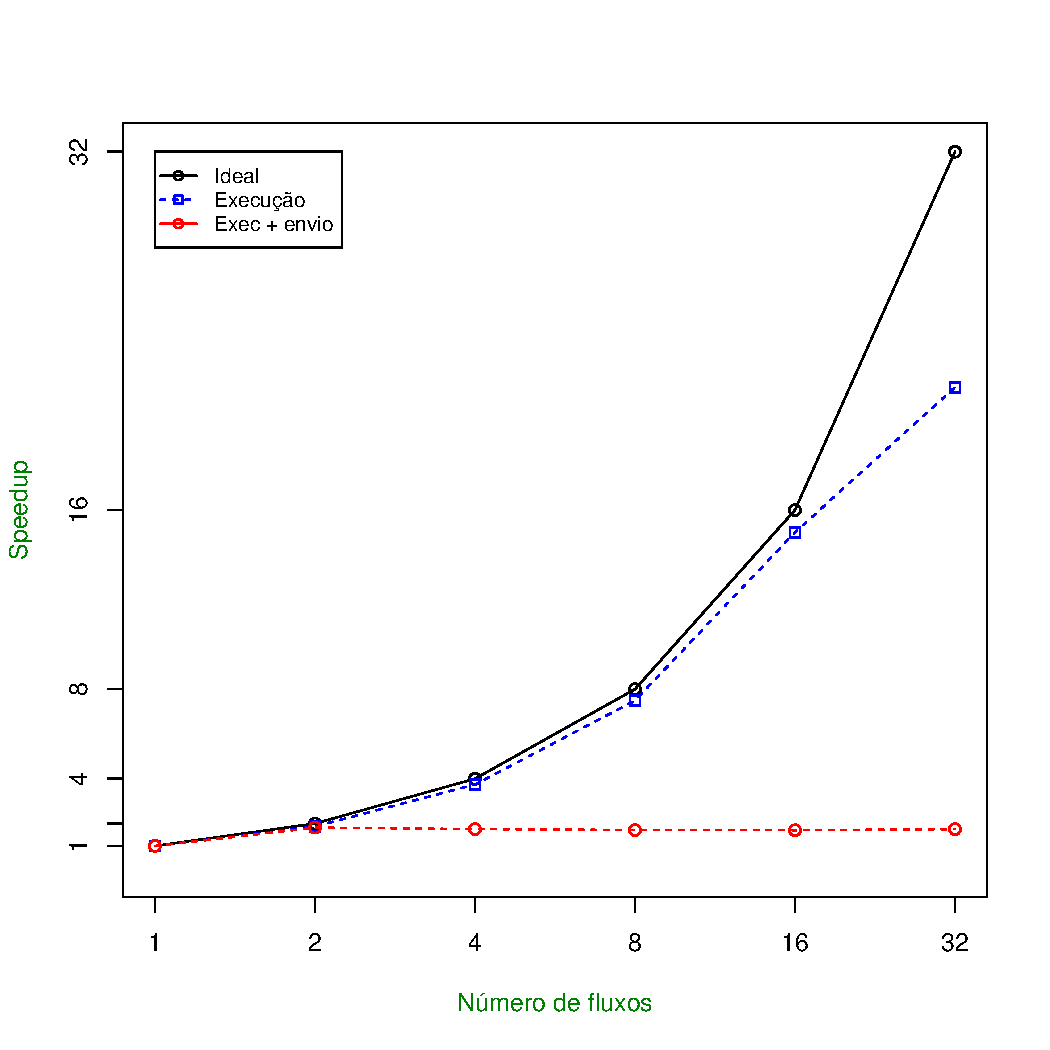
\includegraphics[width=.6\textwidth]{sp.pdf}
\caption{Speedup}
\label{fig:exampleFig1}
\end{figure}

O speedup de execução é bastante expressivo, chegando próximo ao ideal, e pode ser justificado através de uma análise no algoritmo do programa. A estrutura de execução garante que cada fluxo de execução compute parte do problema de maneira independente, isto é, sem interrupções destinadas a comunicação entre os processos, o que caracteriza um problema sem condições de corrida. Esta característica do algoritmo possibilita este grande ganho de desempenho quando desconsiderado o custo do overhead.   

Percebe-se entretanto que o speedup real obtido é baixo, não chegando a atingir 2, isto por que quando se soma o tempo de overhead do envio e recebimento de mensagens entre os processos, o tempo total de execução se torna muito alto. Na figura 2 temos a relação do tempo de inicialização da execução com o número de fluxos de execuções. O tempo da inicialização é a soma do tempo total gasto com alocação dos dados, geração do problema do tamanho dado como parâmetro e o tempo de overhead de envio das mensagens durante a execução do programa, sendo essa, a parte mais longa da inicialização.

\begin{figure}[ht!]
\centering
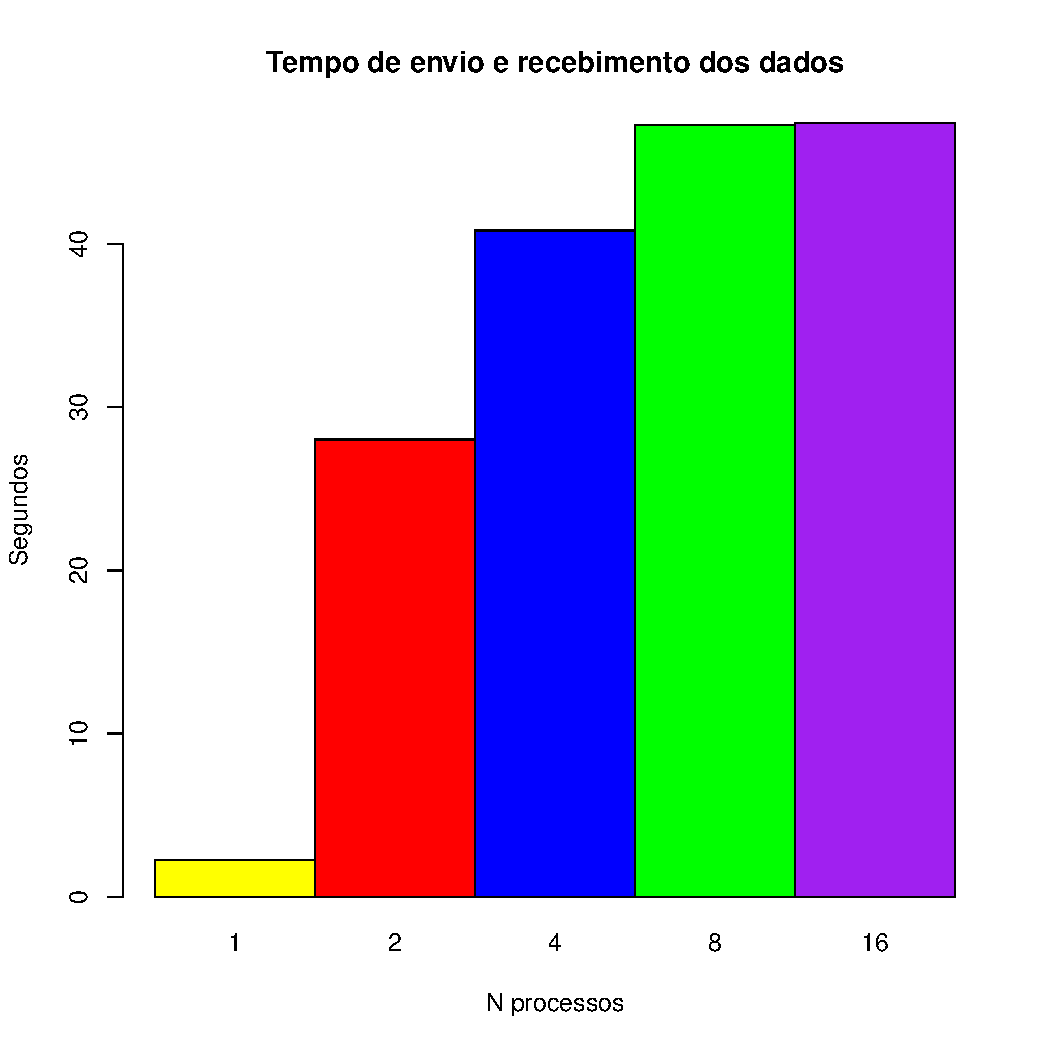
\includegraphics[width=.5\textwidth]{msgs.pdf}
\caption{Custo do overhead}
\label{fig:custooverhead}
\end{figure}

Na execução sequencial e na execução com dois fluxos concorrentes, o tempo de inicialização é perto de 0 pois overhead de envio das mensagens é inexistente neste caso, já que ambas execuções ocorrem em apenas um computador, onde na execução paralela de dois fluxos isto ocorre utilizando dois núcleos do processador. Observa-se que a partir de 4 fluxos concorrentes este tempo se torna muito alto e esta é a causa do speedup real baixo obtido. Apesar do algoritmo possibilitar um speedup semi-ideal a paralelização com memória distribuída acarreta custos adicionais de comunicação que algumas vezes podem ser muitos altos. É importante citar que o tempo de inicialização para a execução com 16 e 32 fluxos concorrentes é quase o mesmo pois para ambas configurações foram utilizadas oito computadores, sendo que na segunda o número de fluxos por computador é dobrado, porém o custo do overhead é praticamente o mesmo já que o número de computadores é o mesmo.


\begin{figure}[ht!]
\centering
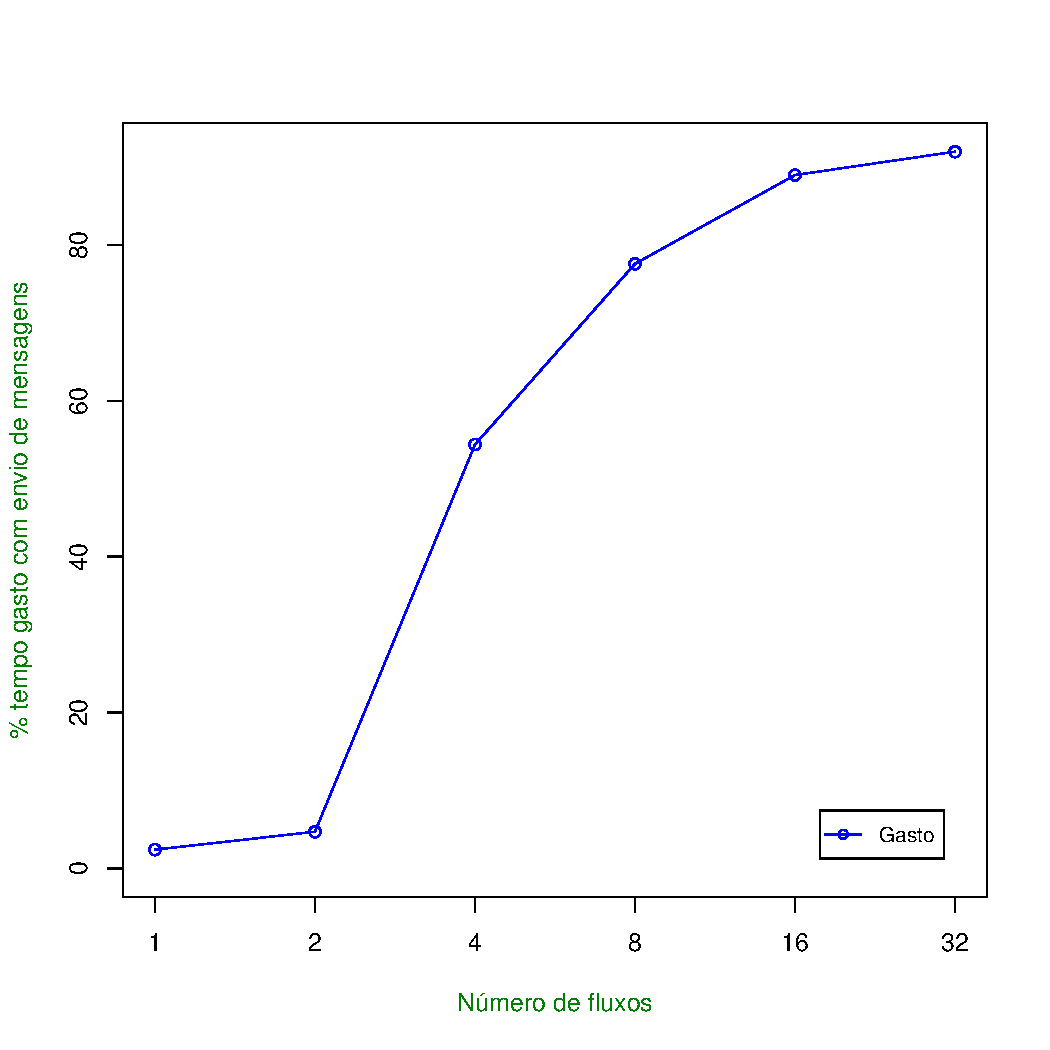
\includegraphics[width=.5\textwidth]{msgsp.pdf}
\caption{Tempo relativo gasto com o envio de mensagens}
\label{fig:desvios}
\end{figure}

Na figura 3, podemos ter a real noção do impacto do custo das trocas de mensagens. Vemos que, conforme a quantidade de fluxos concorrentes e, consequentemente, a de computadores aumenta, o custo das trocas chega a mais de 90\% do tempo. Outra coisa que podemos notar avaliando os gráficos das figuras 2 e 3, é que o tamanho das mensagens não influencia no tempo gasto para as trocas. O quantidade de dados utilizados pelo algoritmo como um todo é o mesmo em todas as execuções, visto que a entrada é a mesma, mas a quantidade de dados utilizados por cada processo diminui conforme a quantidade de fluxos aumenta, pelo fato de que, com mais processos dividindo o trabalho, menos dados são necessários por cada um. Com isso em mente, podemos afirmar que, mesmo com mensagens maiores nas execuções com menos fluxos, isto não é um fator determinante para custo de envio das mensagens, por outro lado, o maior determinante para esse custo é a quantidade de computadores envolvidos na computação.

\section{Conclusão}

Com as análises feitas na seção anterior, podemos afirmar que há um grande ganho no tempo de execução do algoritmo, mostrado pelo gráfico de speedup, mas o gasto com a passagem das mensagens, isto é, dos dados, é muito grande, tornando o ganho real muito pequeno. Mesmo assim, não podemos considerar a implementação deste problema utilizando memória híbrida totalmente ineficiente, pois o ambiente utilizado para os experimentos não é ideal. Quando consideramos a utilização de um cluster de computadores específico para este modelo de paralelização, prevê-se que os resultados obtidos sejam melhores, visto que neste ambiente a comunicação entre os computadores é otimizada para este paradigma paralelo, reduzindo os custos da troca de mensagens, o qual foi o maior limitador do speedup.

No trabalho realizado anteriormente, com memória distribuída, o mesmo limitador do speedup foi encontrado, o grande custo de tempo no envio de dados entre os processos. Pensando nisso uma tentativa para solucionar o problema foi implementada, a ideia era de paralelizar, utilizando pthreads, o envio dos dados, entretanto, o programa apresentou falha crítica ao tentar executar o envio paralelo. Após a realização de uma investigação no problema a causa foi encontrada, a versão do Open MPI instalada no laboratório utilizado nos experimentos não dá suporte a este tipo de operação. Tentativas de solucionar este problema foram realizadas porém nenhuma com sucesso. Desta forma o programa implementado sofre das mesmas limitações graças ao aspecto de memória distribuída.

Conclui-se que a aplicação da técnica de paralelização para modelos de memória hibrida é uma das maneiras mais eficientes de coordenar a computação de algoritmos complexos em diversos sistemas buscando obter melhoras no tempo de execução, entretanto, é sempre importante considerar os custos de comunicação entre os computadores e procurar modelar algoritmos que minimizam esta comunicação. 

\bibliographystyle{sbc}
\bibliography{sbc-template}

\end{document}
